\RequirePackage[T1]{fontenc}
\documentclass[12pt,a4paper,onecolumn,draftclsnofoot]{IEEEtran}
\usepackage[a4paper,margin=1in]{geometry}
\usepackage{times,graphicx,amsmath,booktabs,cite,url}
\usepackage[ruled,linesnumbered]{algorithm2e}
\usepackage{tabularx,array,hyperref}
\hypersetup{hidelinks,pdftitle={CloudCanvas: A Shared Graph Contract for Reviewed AI-Assisted AWS Infrastructure Deployment},pdfauthor={Suhas Kanwar; Suryansh Mahajan; Yaksh Rohilla}}
\setlength{\emergencystretch}{2em}
\graphicspath{{figures/}}
\newcommand{\OverleafProjectLink}{\url{https://www.overleaf.com/project/PLACEHOLDER}}
\newcommand{\CodeRepository}{\url{https://github.com/SuhasKanwar/CloudCanvas}}
\begin{document}
\title{CloudCanvas: A Shared Graph Contract for Reviewed AI-Assisted AWS Infrastructure Deployment}
\author{Group CSE3\_G7: Suhas Kanwar (230603), Suryansh Mahajan (230627),\\
Yaksh Rohilla (230605)\\
School of Engineering \& Technology, BML Munjal University\\
\texttt{suhas.kanwar.23cse@bmu.edu.in}\\
\texttt{suryansh.mahajan.23cse@bmu.edu.in}\\
\texttt{yaksh.23cse@bmu.edu.in}}
\maketitle
\begin{abstract}
Cloud infrastructure design requires users to coordinate service configuration, dependency relationships, deployment order, and resource lifecycle state. Visual editors and language-model assistants can reduce the amount of configuration users write, but a well-formed generated artifact does not necessarily encode a supported or executable architecture. This paper presents CloudCanvas, an AWS-focused prototype that connects a visual workspace and AI-generated drafts through a shared graph contract. The application validates resource structure, permitted attachments, and configuration-reference bindings before a user applies a blueprint; a separate publish action invokes dependency-aware AWS SDK operations and records desired and observed state. The contribution is an implemented integration with an explicit validation boundary, rather than a new language model or a claim of general infrastructure correctness. We evaluate that boundary using 72 deterministic synthetic graph instances, covering 24 valid cases and 48 invalid cases, in three independent Node.js processes. The full contract classifies all 72 cases correctly, compared with 55.56\% for schema-only validation and 77.78\% when reference validation is removed. Mean clone-plus-validation time is 72.9 microseconds per graph, with a sample standard deviation of 14.1 microseconds across processes. Six additional boundary controls remain accepted, illustrating that graph acceptance does not establish output availability, deployment completeness, security, or user intent. These results support layered structural validation on the tested fixtures while motivating separate policy, intent, live-deployment, and human-review evaluations.
\end{abstract}
\begin{IEEEkeywords}
AI-assisted infrastructure, cloud deployment, graph validation, human review, infrastructure as code, visual modeling.
\end{IEEEkeywords}
\noindent\textbf{Overleaf Project Link:} \OverleafProjectLink

\noindent\textbf{Code Repository:} \CodeRepository

\section{Introduction}
Cloud applications depend on relationships among compute, storage, identity, messaging, and delivery services. Provisioning an individual resource is therefore only one part of deployment: identifiers must flow between resources, prerequisites must become ready, and later operations must preserve the distinction between intended configuration and observed state. Infrastructure-as-code systems express these requirements through machine-readable deployment descriptions, while visual modeling tools expose their structure directly. Winery and OpenTOSCA demonstrate that browser-based topology design and topology-driven execution are established approaches, rather than recent consequences of generative AI~\cite{winery2013,opentosca2013}. More recently, language-model research has examined whether natural-language requirements can produce infrastructure artifacts that satisfy explicit intent and actually deploy~\cite{iaceval2024,iacgen2026}. Together, these developments motivate interfaces that connect assistance to an inspectable execution representation.

The practical difficulty is coordinating representations and decisions across that interface. A user may draw a valid-looking connection that the application cannot implement, provide a configuration reference without its dependency edge, or accept an AI response that contains plausible but unavailable identifiers. Errors can arise before any cloud request is made, yet ordinary JSON validation cannot express every graph invariant. Conversely, a graph can satisfy all supported structural rules and still lack an execution role, a deployable function package, or a policy required by the intended workload. An application must communicate which checks it performs and where user decisions remain necessary. Otherwise, successful parsing, visual neatness, and a positive deployment receipt can become misleading substitutes for evidence about infrastructure behavior.

Existing work provides strong foundations but addresses different units of analysis. Modeling languages support richer representations and formal properties; IaC benchmarks measure generated code against requirements or deployment outcomes; commercial platforms combine visual components, contracts, and automated workflows~\cite{doml2024,multi2025,massdriver}. CloudCanvas does not resolve the limitations of these approaches generally. The narrower gap investigated here is how a single application-level graph contract can connect manual editing, structured AI drafts, persistence, and a bounded SDK execution path, and what additional structural faults its layers detect. This formulation avoids comparing a prototype's feature inventory with another system's measured generation scores. It also makes the evaluation feasible without claiming that a local graph experiment measures provider permissions, operational safety, or user productivity.

We present CloudCanvas as a concrete AWS-focused implementation of this workflow. Users create resource nodes manually or obtain an AI blueprint, inspect its configuration, and explicitly apply it to a saved sketch. Publishing is a separate action. Express controllers then perform ownership and deployment checks, build an execution order, resolve source outputs, and invoke resource-specific AWS SDK handlers. PostgreSQL records sketches, conversations, configurations, resource identifiers, statuses, and deployment outcomes. The architecture deliberately constrains the supported representation: eleven resource types and four attachment pairings are implemented. This bounded scope enables explicit rules but limits the architectures that can be expressed. It does not provide unrestricted cloud automation or a new infrastructure language standard.

The paper addresses two research questions. \textbf{RQ1:} On a declared synthetic conformance corpus, how much does the complete graph contract improve rejection of structural faults over schema-only validation and a schema-plus-topology ablation? \textbf{RQ2:} What local processing cost accompanies these checks, and which deliberately constructed boundary conditions remain outside their acceptance predicate? The first question concerns conformity to implemented representation rules; the second examines cost and limits. Neither asks whether the language models generate better architectures than competing tools. We make the following concrete contributions:
\begin{itemize}
\item An implementation description connecting an editable AWS graph, reviewed AI proposals, persisted state, and dependency-aware SDK execution.
\item A formal account of the shared contract's structural acceptance boundary, including the separation between reference binding and runtime output resolution.
\item A reproducible 72-instance conformance experiment, three independent process runs, two reduced-validation comparisons, and six boundary controls, with raw results and vector figures.
\end{itemize}
The remaining sections review related work, formulate the problem, explain the implementation and experiment, analyze the results, and discuss the limits of the supported claims.

\section{Related Work}
\subsection{Visual and Model-Driven Infrastructure}
Winery implements a topology editor, reusable component definitions, and a repository for TOSCA descriptions~\cite{winery2013}. Its demonstration establishes the feasibility of visual typed composition, while deployment execution is delegated to other components. OpenTOSCA supplies a runtime for packaged application topologies, implementation artifacts, and management plans~\cite{opentosca2013}. These systems are relevant because they separate the representation a user edits from the mechanism that executes it. They prevent a broad novelty claim for CloudCanvas's canvas or deployment graph. Their demonstration evidence also should not be interpreted as a latency baseline for an AWS SDK application developed in a different environment.

CAMEL extends modeling beyond topology to requirements, providers, metrics, scaling, and runtime instances~\cite{camel2019}. Its practitioner study considers perceived usability, rather than proving a universal deployment-speed advantage. The Essential Deployment Metamodel extracts common concepts from deployment technologies and explains limits in mapping among them~\cite{edmm2020}. This highlights a central restriction of CloudCanvas: resource relationships have application-specific meaning, and a visual line is not automatically portable across tools. DOML further separates application, abstract-infrastructure, and concrete-infrastructure models, generates IaC, and uses a Z3-backed checker for model properties~\cite{doml2024}. CloudCanvas's schema and graph checks are narrower than this property-verification approach. Its smaller representation is a design choice whose usability consequences require evidence.

\subsection{AI Generation, Intent, and Deployability}
IaC-Eval provides 458 AWS/Terraform scenarios paired with intent specifications, using a speculative deployment graph and OPA checks to distinguish syntactic acceptance from requested behavior~\cite{iaceval2024}. CloudCanvas currently lacks an equivalent independent intent oracle. Multi-IaC-Eval examines changes to existing templates across multiple formats, combining static tools and semantic review~\cite{multi2025}. Its exclusion of live deployment testing is material: high static compliance cannot be relabeled provider success. It also motivates preservation checks for future graph editing, because CloudCanvas's current AI application action replaces a complete graph rather than performing a verified incremental mutation.

TerraFormer uses policy-guided verifier feedback for dataset construction and model fine-tuning~\cite{terraformer2026}. This is a training-and-evaluation contribution that CloudCanvas does not implement. IaCGen instead emphasizes iterative formatting, syntax, and actual deployment feedback over 153 CloudFormation scenarios~\cite{iacgen2026}. Its results depend on the number of attempts, underlying models, and the definition of success. Neither benchmark is directly comparable to classification of synthetic graph fixtures. The preliminary cloud-agent study compares SDK, command-line, Terraform, and web agents on Azure VM tasks, then motivates synchronized state, policy enforcement, and human supervision~\cite{agents2025}. Differences in underlying models and task scope limit interpretation of its operational comparisons.

\subsection{Comparison and Research Gap}
Table~\ref{tab:related} compares six representative papers on the dimensions most relevant to this study. It records the type of evidence each contributes, rather than treating absent discussion of a feature as proof that the feature is unsupported. The remaining four papers supply complementary context on executable topology, runtime models, deployment abstractions, and agent supervision.
\begin{table}[t]
\caption{Representative related work and its relevance to CloudCanvas.}
\label{tab:related}
\centering\footnotesize
\begin{tabularx}{\linewidth}{p{.17\linewidth}XXX}
\toprule
Work and problem & Approach & Evaluation and result & Limitation and relevance \\
\midrule
Winery~\cite{winery2013}: topology design & Typed visual editor and repository & Moodle on two EC2 VMs demonstrates composition & Establishes canvas prior art with no controlled outcome comparison \\
DOML~\cite{doml2024}: model correctness & Model layers and Z3 property checks & Modified WordPress case exposed mapping and network errors & Limited generality across cases, but stronger model invariants \\
IaC-Eval~\cite{iaceval2024}: generated intent & Terraform plan with a policy oracle & 458 scenarios. Historical GPT-4 pass@1 of 19.36\% & AWS/Terraform scope motivates separate intent checks \\
Multi-IaC-Eval~\cite{multi2025}: template edits & Static and semantic checks & 337 CloudFormation, 171 Terraform, and 191 CDK templates & No live deployment test. Motivates preservation checks for edits \\
TerraFormer~\cite{terraformer2026}: generation quality & Policy feedback and fine-tuning & IaC-Eval correctness rose from 15.50\% to 31.44\% for the reported 14B condition & Depends on policy coverage. Motivates actionable diagnostics \\
IaCGen~\cite{iacgen2026}: deployability & Iterative cloud feedback & 153 scenarios. First-attempt deployability of 20.8--30.2\% across six models & Provider and model dependence calls for separate lifecycle measures \\
\bottomrule
\end{tabularx}
\end{table}
Commercial prior art strengthens this qualification. Massdriver documents visual composition of IaC bundles, JSON Schema input/output contracts, dependency checks, and managed deployment pipelines~\cite{massdriver}. Accordingly, visual composition plus schemas plus deployment is not, by itself, an original contribution. The specific contribution here is a source-grounded account and controlled conformance evaluation of CloudCanvas's shared intermediate graph and reviewed execution workflow. Its comparison baselines remove validation layers within that same representation. This isolates a tractable question while leaving usability, AI generation accuracy, enterprise governance, and live cloud reliability as separate evaluation targets.


The studies also differ in how they establish the expected result. Winery and OpenTOSCA demonstrate representative application workflows. CAMEL collects practitioner judgments. DOML checks declared properties on application models. IaC-Eval and TerraFormer depend on requirements encoded as policies, and IaCGen adds feedback from attempted deployment. Each method creates visibility into a different part of the system. A practitioner rating cannot explain which graph errors an implementation detects. A formal check of a particular property cannot establish that a user asked for that property. A successful deployment cannot establish that the resulting configuration reflects every requested restriction. These differences inform both the structure of the present experiment and its limitations.

Table~\ref{tab:related} therefore gives the reported benchmark values only with their original denominators and comparison conditions. For example, TerraFormer's gain refers to its tested model and verifier pipeline, and IaCGen's first-attempt rates describe actual deployment attempts for a different artifact format. Neither number provides a target for the percentage of labeled structural fixtures classified correctly here. A future CloudCanvas study could adapt the underlying evaluation techniques by writing independent requirement predicates, making review decisions observable, and checking actual resource outcomes against those predicates. Such a study would address a different research question from the current layer-by-layer conformance experiment.

\section{Background / Problem Formulation}
A sketch is a directed attributed graph $G=(V,E,\tau,c,p)$, where $V$ contains resource nodes, $E\subseteq V\times V$ contains dependency edges, $\tau$ maps nodes to supported resource types, $c$ stores configuration objects, and $p$ stores canvas positions. An edge $(u,v)$ means that $u$ supplies a supported provisioning dependency to $v$; it does not denote arbitrary network communication. The implemented relation set contains key-pair-to-EC2, security-group-to-EC2, IAM-role-to-Lambda, and S3-to-CloudFront attachments. A node may also be independent. A configuration reference names a source node and one output field, using the exact form \texttt{\$\{source.field\}}.

The input is either a manually assembled graph or a structured AI proposal. The immediate output is an accepted, normalized draft or a diagnostic explaining rejection. A later publish request supplies an owned AWS connection and attempts supported operations. These are different outputs: acceptance into the workspace is not certification that execution will succeed. JSON Schema supplies the document-shape vocabulary~\cite{jsonschema2022}, and Ajv executes those checks with the application's defaults and validation settings~\cite{ajv}. Separate graph rules express constraints that document shape alone cannot capture.

Let $S(G)$ denote schema validity, $T(G)$ denote node/edge and topology validity, and $R(G)$ denote configuration-reference syntax and direct-source binding. The shared acceptance condition is
\begin{equation}
 A(G)=S(G)\land T(G)\land R(G).
 \label{eq:accept}
\end{equation}
For every recognized reference $r=(u,k)$ in node $v$, the reference layer requires
\begin{equation}
 u\in\operatorname{Pred}_{G}(v),\qquad
 \operatorname{Pred}_{G}(v)=\{w:(w,v)\in E\}.
 \label{eq:reference}
\end{equation}
Here $k$ is a syntactically permitted output token. Equation~\ref{eq:reference} does not establish that the runtime output actually contains $k$; resolution checks that later. This distinction is deliberately exercised by a boundary control.

The formulation assumes authenticated application access for protected operations and a supported resource subset. It excludes arbitrary AWS coverage, multi-cloud translation, formal security proofs, workload health, model training, and production governance. Configuration may remain incomplete in a draft because users must sometimes choose account-specific values after generation. The engineering problem is therefore to preserve a consistent, inspectable draft representation while keeping later deployment preconditions explicit. The experimental problem is narrower still: measure acceptance decisions against declared structural expectations, without converting those expectations into claims about intent or provider execution.

\section{Proposed Methodology}
\subsection{Architecture and the Shared Representation}
Fig.~\ref{fig:architecture} shows the application components and their principal relationships. A Next.js workspace exposes the resource canvas, configuration forms, saved sketches, resource observations, and conversation interface. Express owns protected application APIs, persistence coordination, and AWS operations. FastAPI hosts the LangGraph workflow, while PostgreSQL stores the application's durable records. The shared TypeScript graph contract is imported by the client and server; it is not an HTTP service and is not directly imported by Python. Separating it from either interface allows returned AI drafts and user-imported graph descriptions to meet the same application acceptance boundary~\cite{cloudcanvas}.
\begin{figure}[t]
\centering
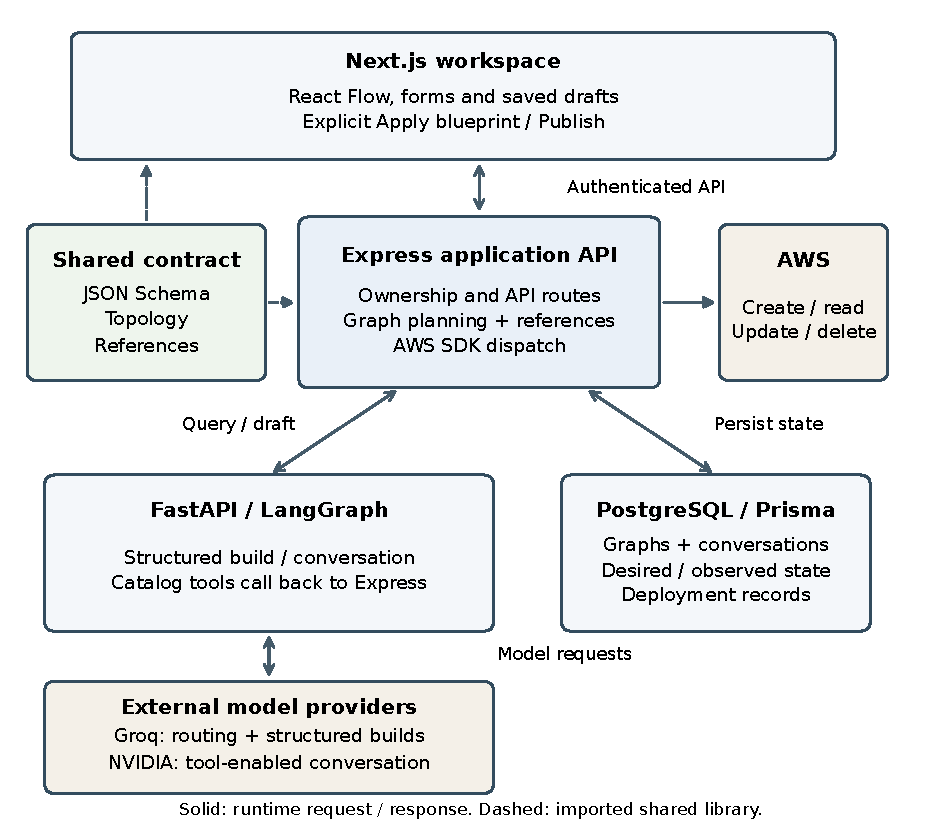
\includegraphics[width=.98\linewidth]{architecture.pdf}
\caption{CloudCanvas architecture. Solid connections denote runtime communication; dashed connections denote use of the shared TypeScript library. AI returns advice or drafts, while application code controls AWS mutation.}
\label{fig:architecture}
\end{figure}
The contract declares supported service types, configuration schemas, edge compatibility, graph diagnostics, and reference rules. Python uses separate Pydantic definitions for structured responses, so the server validates returned builds again rather than assuming language-level equivalence. This duplicates some type knowledge but creates an explicit runtime trust boundary. JSON Schema provides an inspectable document definition, and Ajv is configured with defaults, all-error reporting, and non-strict schema compilation~\cite{jsonschema2022,ajv}. Those choices support normalization and useful diagnostics. They do not turn optional draft fields into deployment-ready configuration.

\subsection{Layered Graph Validation}
Algorithm~\ref{alg:validation} describes the logical validation sequence. Schema checking first rejects unsupported document shapes and values. The topology stage then checks unique node identifiers, known edge endpoints, self-edges, compatible attachments, duplicate edges, and the single-origin constraint for CloudFront. It derives predecessor sets and a topological order. Reference validation recursively traverses configuration values, accepting reference strings only when their syntax is exact and their source is a direct predecessor. This explicit association prevents an apparently meaningful reference from bypassing the graph's dependency representation.
\begin{algorithm}[t]
\caption{Validate a proposed CloudCanvas graph}
\label{alg:validation}
\KwIn{Candidate graph $G$; shared schema; permitted type relation set}
\KwOut{Normalized graph and topological order, or diagnostics}
Check $S(G)$; return diagnostics if schema validation fails\;
Require unique identifiers for every node in $V$\;
Initialize predecessor sets and in-degree counters\;
\ForEach{edge $(u,v)\in E$}{
Require known distinct endpoints and a permitted type pairing\;
Reject duplicate edges and multiple CloudFront origins\;
Record the predecessor and increment the target in-degree\;
}
Compute a topological order; reject if it does not cover $V$\;
\ForEach{configuration value containing reference syntax}{
Require the exact reference form and extract $(u,k)$\;
Require $u\in\operatorname{Pred}_{G}(v)$ for its consuming node $v$\;
}
\Return{accepted normalized graph and order}\;
\end{algorithm}
For an accepted dependency edge, the order $\pi$ must satisfy
\begin{equation}
 (u,v)\in E\ \Longrightarrow\ \pi(u)<\pi(v).
 \label{eq:order}
\end{equation}
The notation $\pi(v)$ denotes a node's position in the execution ordering. The supported type-pair relation is itself acyclic, so the tested cyclic fixture also violates compatibility; the experiment does not isolate the cycle-detection branch. Although the planner follows a Kahn-style structure, its current per-edge node searches and array-based queue can introduce $O(|V||E|+|V|^2+B)$ work, where $B$ denotes configuration traversal size. We consequently avoid a general linear-time or large-graph scalability claim.

\subsection{Reviewed AI Drafting and Workspace Persistence}
The active LangGraph workflow routes AWS construction requests to a structured Groq branch and general conversation to a NVIDIA branch with tool calls~\cite{langgraph}. Tools supply resource-support guidance, web search, and an authenticated callback for AWS catalog choices. The conversation controller includes bounded catalog context and prior conversation text, but does not automatically serialize the complete current canvas into the model prompt. Provider clients are instantiated lazily; a defined alternative Llama wrapper is not part of the active graph. Model outputs are text advice or draft graphs, not unrestricted cloud mutation commands.

Fig.~\ref{fig:workflow} illustrates the user-facing path from proposal to observed outcome. Applying a blueprint and publishing infrastructure are separate decisions. Accepted blueprint replacement runs transactionally, remaps persisted node identifiers and configuration references, and is blocked while associated resources remain non-terminated. Manual canvas changes use incremental APIs and queued debounce persistence; undo and redo operate on editor snapshots. The separation makes drafts inspectable, but a full replacement is not a verified incremental editing engine. The paper evaluates validation before these application decisions. The effectiveness of user review would require a separate study.
\begin{figure}[t]
\centering
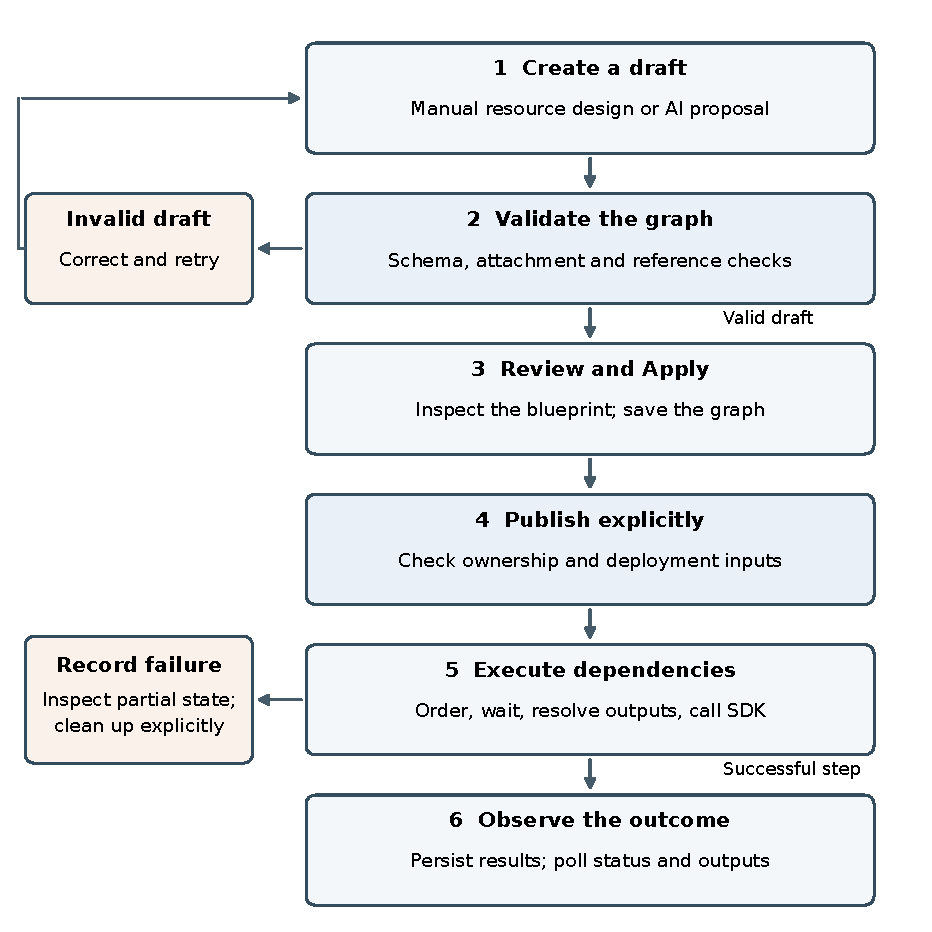
\includegraphics[width=.96\linewidth]{workflow.pdf}
\caption{Reviewed workflow, including rejection before application and explicit handling of partial execution failure. Publish performs additional checks beyond draft acceptance.}
\label{fig:workflow}
\end{figure}

\subsection{Execution, Observation, and Cleanup}
Publishing checks the owned sketch and connection, validates supported deployment inputs, decrypts the connection credentials, and constructs the execution order. For each node, the controller waits for direct dependencies, resolves configuration references against stored or refreshed outputs, and dispatches the appropriate AWS SDK operation~\cite{awssdk}. Unlike draft reference validation, resolution checks the requested output field's availability. Resource records distinguish desired configuration, observed state, external identifiers, management ownership, and errors. Deployment records preserve requests, outcomes, and timestamps. This accounting makes partial progress visible but is not a transaction spanning AWS and PostgreSQL.

Most successful create returns initially become application-level running records; CloudFront remains provisioning until later observation. The editor triggers status refresh periodically, and dependent operations explicitly wait for required readiness. Therefore, an accepted API response, the application's running label, and workload health remain different observations. A user can inspect outputs or request cleanup. Bulk cleanup reverses dependency order and stops at a pending or failed result; adopted resources are detached locally while managed resources are deleted. S3 content/version deletion and forced ECR deletion are consequential operations, and asynchronous CloudFront cleanup depends on subsequent refresh calls.

This prototype intentionally retains important operational limitations. Execution runs within an Express request without a durable worker, atomic per-sketch reservation, automatic rollback, or general idempotency guarantee. Some error paths can leave pending deployment receipts. Normal node configuration updates are blocked for live resources even though update dispatchers exist. Express protects sketch and connection APIs with JWT ownership checks, but the present Google profile exchange and FastAPI service boundary require further hardening. These limitations are part of the described implementation, not capabilities supplied implicitly by the libraries. Docker Compose packages the client, server, AI service, and database with internal networking and migration startup~\cite{compose}; packaging alone does not address these lifecycle and security gaps.

\section{Experimental Setup}
\subsection{Corpus and Compared Pipelines}
The experiment uses synthetic conformance fixtures stored with the paper, rather than model outputs, production architectures, or an existing benchmark's task corpus. Eight base patterns cover all eleven supported node types and the four permitted attachment pairings. Three naming/position variants produce 24 valid instances. Eight shape mutations, eight topology mutations, and eight reference mutations are each instantiated twice, producing 48 invalid instances. The resulting 72-instance corpus has 16 examples per fault category. Repeated variants are closely related, so the instance count must not be interpreted as 72 independently sampled architecture tasks.

The schema-only baseline runs Ajv with the application's schema and options. The schema-plus-topology ablation adds the exported graph planner but omits reference traversal. The full-contract condition invokes the actual exported validator. All conditions receive fresh cloned inputs, preventing defaults or earlier normalization from affecting later decisions. Fault expectations are specified when constructing fixtures, and assertions verify that the intended corpus and supported-type coverage are present. Six separate boundary controls test accepted drafts with issues beyond this structural predicate; they are not counted as structural false accepts.

\subsection{Execution Environment and Parameters}
Three fresh Node.js processes execute the same corpus. The pipeline order rotates deterministically across processes, and every condition receives 20 warm-up passes before 50 timed passes. Timing includes input cloning, validation, and error handling, but excludes module import and schema compilation. It therefore measures steady-state local gate processing rather than startup or deployment latency. The raw JSON records environment information, decisions, run order, corpus settings, source digests, and individual measurements.

Table~\ref{tab:parameters} lists the measured environment and fixed settings. No model is trained or queried, so training splits, generation temperatures, and random seeds are inapplicable to this experiment. Application model settings remain source-inspectable but do not explain the measured validation outcomes.
\begin{table}[t]
\caption{Recorded offline experiment parameters.}
\label{tab:parameters}
\centering\small
\begin{tabularx}{\linewidth}{lX}
\toprule
Parameter & Value \\
\midrule
Platform & Linux, x86-64; kernel 7.1.5-arch1-2 \\
Processor / memory & Intel Core i5-1135G7, 8 logical CPUs; 31.08 GiB RAM \\
Runtime / validator & Node.js 22.23.1; Ajv 8.20.0; YAML 2.9.0 \\
Independent runs & 3 fresh processes; rotated pipeline order \\
Corpus & 24 valid + 48 invalid instances; 6 separate boundary controls \\
Warm-up / measurement & 20 / 50 complete corpus passes per pipeline and process \\
Timing unit & Microseconds per graph, including cloning and exceptions \\
Randomness / provider access & Deterministic fixtures; no seed, model calls, or AWS requests \\
\bottomrule
\end{tabularx}
\end{table}

\subsection{Metrics and Reproduction}
For $N$ labeled structural cases, classification accuracy and invalid false-acceptance rate are
\begin{equation}
 \operatorname{Acc}=\frac{\mathrm{TP}+\mathrm{TN}}{N},\qquad
 \operatorname{FAR}=\frac{\mathrm{FP}}{N_{\mathrm{invalid}}}.
 \label{eq:metrics}
\end{equation}
Here TP denotes accepted valid cases, TN rejected invalid cases, and FP accepted invalid cases. False rejections are reported separately because stricter validation must not silently discard supported drafts. Mean latency and sample standard deviation use the three per-process measurements, with denominator $n-1$ for variance and $n=3$. Correctness is expected to be deterministic; timing variability reflects the shared workstation. The repository supplies the corpus generator, raw decisions, summary CSV, figure generator, and commands for reproduction~\cite{cloudcanvas}.


Before timing, the runner checks that each valid fixture is accepted and each structurally invalid fixture is rejected by the full contract. These assertions detect drift between the declared test cases and the studied version. They also constrain the interpretation of the perfect full-contract result: fixture construction targets known contract behavior. The reduced pipelines receive the same cases and options, so the experiment tests whether suppressing a validation layer changes which errors cross that boundary. Reproduction should compare case-level decisions first and treat the recorded time values as machine-specific observations.

\section{Results and Analysis}
\subsection{RQ1: Structural Fault Rejection}
Table~\ref{tab:results} reports the three pipeline conditions using the same labeled corpus. The full contract classifies all 72 instances correctly in each process, whereas schema-only validation classifies 40 correctly and schema plus topology classifies 56 correctly. This corresponds to accuracies of $100.00\%$, $55.56\%$, and $77.78\%$, respectively, with zero sample standard deviation for classification across runs. These are conformance results on constructed instances. They are not estimates of AI generation accuracy, production failure probability, or correctness over arbitrary infrastructure.
\begin{table}[t]
\caption{Three-process results. Values with uncertainty show mean $\pm$ sample SD; timing includes cloning. Bold denotes the highest structural accuracy on this corpus.}
\label{tab:results}
\centering\footnotesize
\begin{tabular}{lrrrr}
\toprule
Pipeline & Accuracy (\%) & False accepts / 48 & False rejects / 24 & Time ($\mu$s) \\
\midrule
Schema only & $55.56 \pm 0.00$ & $32 \pm 0$ & 0 & $41.3 \pm 8.9$ \\
Schema + topology & $77.78 \pm 0.00$ & $16 \pm 0$ & 0 & $57.6 \pm 26.0$ \\
Full contract & $\mathbf{100.00 \pm 0.00}$ & $0 \pm 0$ & 0 & $72.9 \pm 14.1$ \\
\bottomrule
\end{tabular}

\end{table}
Schema-only validation rejects the 16 shape/type faults but accepts all 32 invalid topology or reference instances. Its false-acceptance rate among invalid cases is therefore $66.67\%$. Adding topology checks rejects another 16 cases and reduces that rate to $33.33\%$. The complete contract rejects the remaining reference faults and has no structural false accepts in this corpus. Every condition accepts all 24 labeled valid cases, so the observed gain does not trade away any of the corpus's supported positives. This does not establish the absence of false rejections on other valid architectures or configuration combinations.

Fig.~\ref{fig:errors} breaks the errors down by fault class. The pattern follows the constraints removed by the ablations: document-shape rules cannot detect duplicate graph identifiers or unsupported relationships, while topology checks alone cannot inspect configuration strings for unbound references. Each bar summarizes 16 constructed cases, and the same counts occur in every process. The result supports retaining all three layers in the application's acceptance boundary. It does not demonstrate that the selected fault classes occur with the same frequency in real AI responses or user-created sketches.
\begin{figure}[t]
\centering
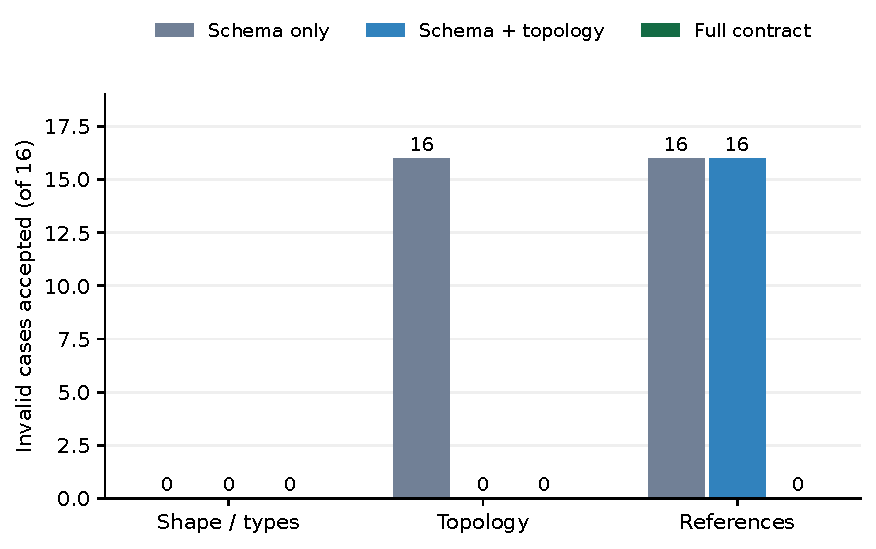
\includegraphics[width=.95\linewidth]{validation-errors.pdf}
\caption{Invalid instances accepted by fault category and validation pipeline. Each category contains 16 cases; counts are identical across the three processes.}
\label{fig:errors}
\end{figure}
The ablation is particularly informative for configuration references. The middle pipeline still verifies that a graph has compatible, known endpoints and an execution ordering, yet it accepts references without the required source binding. Thus an accepted topology is insufficient to connect configuration values to that topology. Conversely, a schema-valid string that resembles an output expression has no operational meaning until the source relationship and later output availability are checked. The improvement measured here is fault detection added by these particular layers, not a new property of topological sorting or schema validation.


The corpus makes the effect of each layer countable. Relative to schema alone, adding topology checks changes the decisions on 16 of the 72 instances, raising accuracy by 22.22 percentage points. Reference analysis changes a different 16 decisions by the same amount. The pipeline retains the shape filter throughout, so the gains are additive for these assigned categories. That arithmetic depends on equal category sizes and the construction of single dominant faults. In an observed mixture of defects, errors could overlap and the gains would depend on which defects occur most often. For instance, a missing source node may cause a graph error before a later configuration reference is even examined. The experiment describes the final rejection decision and does not measure the completeness of the diagnostic messages.

Acceptance of the valid fixtures also needs qualification. A positive fixture for a service demonstrates at least one admitted configuration pattern. It does not test every combination of optional parameters, every account setting, or every interaction among supported services. The recorded corpus and case-level decisions allow a reader to identify exactly which patterns were exercised. A suite drawn from naturally occurring authoring errors would provide complementary evidence about which checks matter most in everyday use.

\subsection{RQ2: Processing Cost and Boundary Behavior}
The measured clone-plus-validation means are $41.3\pm8.9$ microseconds for schema only, $57.6\pm26.0$ microseconds for schema plus topology, and $72.9\pm14.1$ microseconds for the full contract. Fig.~\ref{fig:latency} presents these per-process statistics with error bars. The complete pipeline performs additional graph traversal, reference scanning, and exception handling, which explains the direction of the mean differences. The substantial variability and only three processes do not support a statistical claim about the exact marginal cost or a universal performance ranking. All measurements concern small fixtures after warm-up, with no network communication.
\begin{figure}[t]
\centering
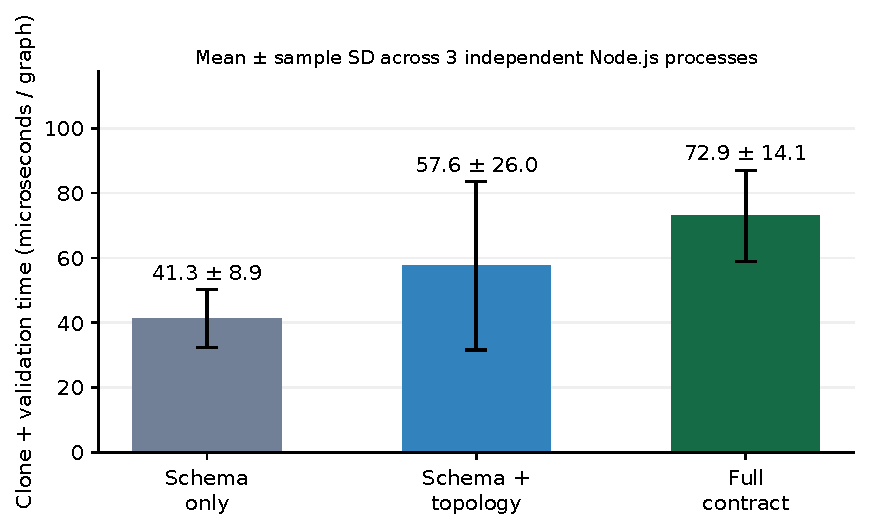
\includegraphics[width=.95\linewidth]{validation-latency.pdf}
\caption{Mean local validation cost and sample SD across three fresh processes. Error bars describe process-level variability, not uncertainty in cloud-deployment latency.}
\label{fig:latency}
\end{figure}
Table~\ref{tab:boundary} records six controls that the full graph contract accepts in each process. They deliberately probe distinctions outside the structural labels: output-field existence, deployment completeness, additional publish restrictions, execution-role trust, identifier availability, and external user requirements. Their acceptance is not hidden inside the structural accuracy score. Instead, it explains why that score cannot be used as a global safety percentage.
\begin{table}[t]
\caption{Accepted boundary controls and the check still needed. All six pass graph validation; none was deployed.}
\label{tab:boundary}
\centering\small
\begin{tabularx}{\linewidth}{lX}
\toprule
Control & Interpretation / additional check \\
\midrule
Unknown output field & Direct source exists; runtime output resolution must check the field. \\
Incomplete Lambda draft & Draft schema permits missing execution fields; publish must reject incompleteness. \\
Public S3 / CloudFront origin & Graph shape permits the setting; publish preflight rejects the combination. \\
Wrong IAM trusted service & Type-compatible attachment alone does not prove execution-role suitability. \\
Unverified AMI literal & A string does not prove an identifier exists in the selected region. \\
Unmet SNS requirement & A valid S3 graph does not satisfy an independent request for SNS. \\
\bottomrule
\end{tabularx}
\end{table}
The six controls are explanatory examples, not a measured distribution of operational defects. Several require information intentionally unavailable to the offline validator, while others belong to later application checks or a missing intent/policy oracle. No AWS deployment failure was observed here because no AWS operation was attempted. Together, the controls and ablations answer RQ2: the additional local checks have a measurable processing cost and a clearly limited acceptance meaning. A downstream study should evaluate publish preconditions, provider execution, intent satisfaction, and cleanup with separate denominators rather than extending the present $100\%$ conformance result to those outcomes.


The timing means should be interpreted alongside this decision analysis. The difference between the schema-only and full-contract means is 31.6 microseconds per graph in the recorded runs. The timer includes creating a fresh input and catching rejection exceptions, so both the work performed and the proportion of inputs that throw can influence it. It would be premature to assign the entire difference to reference traversal or extrapolate it to a user-facing response time. A dedicated scaling experiment would vary graph size and configuration depth while holding the acceptance mix constant, then report preparation, validation, and diagnostic costs separately.

\section{Discussion}
The results support a practical design choice: a shared representation should carry relationship and reference invariants in addition to field types. Without those checks, a structurally plausible draft can cross the application boundary even though its dependency meaning is inconsistent. Explicit user review remains useful as an interface design, but this study does not measure whether users notice such problems or whether the interface improves their decisions. Human approval cannot substitute for service authentication, authorization, or independent policy verification.

Construct validity is the principal limitation. The oracle defines correctness as conformity to the tested graph rules; it does not measure workload requirements or operational security. Internal validity is limited by a small deterministic corpus, related naming/position variants, and fixtures designed with knowledge of the representation. The cycle example also violates type compatibility, so it cannot independently demonstrate cycle-check coverage. Boundary controls expose selected limitations but do not exhaust them. Timing is affected by runtime behavior, input cloning, exception cost, host scheduling, and unpinned processor frequency.

External validity is similarly restricted. The corpus covers eleven declared types and four pairings, not arbitrary architectures or provider behavior. No model-generated distribution, expert annotation study, competitor trial, live deployment run, or large-scale graph experiment is included. Three fresh processes provide repeated execution and descriptive variability, not three independently collected datasets. Paper benchmark results and vendor capabilities therefore remain contextual evidence rather than directly comparable measurements~\cite{iaceval2024,iacgen2026,massdriver}.

Operational implications also deserve restraint. Request-driven publishing, incomplete receipt finalization, delegated tokens, and missing service-boundary hardening remain engineering gaps. A system with a correct draft validator can still create duplicate resources, leave orphaned state, or authorize an unsafe action if other layers fail. Ethical evaluation should accordingly avoid unbounded cloud spend, protect credentials and conversation data, and record cleanup obligations. The present study uses synthetic identifiers and makes no provider requests. Future studies involving users should obtain consent and independently define task success, while live cloud experiments should preserve resource inventories, failure records, and teardown evidence.

\section{Conclusion and Future Work}
CloudCanvas implements an AWS-focused workflow that connects an editable resource graph, structured AI proposals, explicit application and publish decisions, persisted lifecycle records, and dependency-aware SDK operations. The integration is the system contribution; visual cloud modeling, topology execution, and AI-assisted infrastructure generation remain established prior work. The paper's experiment examines the shared graph contract rather than attributing broad correctness or productivity gains to the interface.

For RQ1, the full contract correctly classifies all 72 synthetic conformance instances, compared with $55.56\%$ for schema-only validation and $77.78\%$ for the schema-plus-topology ablation, with no observed false rejections. For RQ2, full validation costs $72.9\pm14.1$ microseconds per small graph across three fresh processes, while all six selected boundary controls remain accepted, demonstrating that the structural predicate has limited operational meaning. These numbers describe the supplied fixtures and workstation; they do not establish superiority in live deployment, security, intent satisfaction, or usability.

Three concrete directions follow. First, add independent graph-intent and policy oracles, then evaluate catalog grounding and review with matched models and held-out tasks. Second, make execution durable through atomic operation reservation, idempotency, complete failure finalization, and interrupted-operation recovery. Third, conduct bounded live-AWS lifecycle and controlled user studies that report readiness, cleanup, unsafe approvals, and correction effort separately. Those studies would test whether the implemented workflow produces benefits beyond the conformance boundary demonstrated here.


\section*{AI-Use Declaration}
This author-review draft contains AI-assisted manuscript drafting, literature synthesis, experiment-script development, and figure preparation. The recorded experimental values were produced by the supplied executable scripts; they are not invented model outputs. The named authors must verify the sources, reproduce the experiments, revise the text, and approve the final submission. No similarity or AI-content percentage is certified by this manuscript, and the institution's required reports have not been produced.

\section*{Author Contributions}
The following manuscript responsibilities are assigned for team confirmation; they do not independently establish historical implementation ownership. Suhas Kanwar: system architecture, software-description verification, and manuscript integration. Suryansh Mahajan: related-work synthesis, reference verification, and technical editing. Yaksh Rohilla: experimental reproduction, result and figure verification, and final consistency review. All three authors are responsible for approving the final claims and the submitted version.

\bibliographystyle{IEEEtran}
\bibliography{references}
\end{document}
